%& -shell-escape

%% Copyright (c) 2010-2012, Илья w-495 Никитин
%%
%% Разрешается повторное распространение и использование
%% как в виде исходного кода, так и в двоичной форме,
%% если таковая будет получена, с изменениями или без,
%% при соблюдении следующих условий:
%%
%% * При повторном распространении исходного кода
%% должно оставаться указанное выше уведомление
%% об авторском праве, этот список условий
%% и последующий отказ от гарантий.
%% * Ни имя w-495, ни имена друзей или консультантов
%% не могут быть использованы в качестве поддержки
%% или продвижения продуктов, основанных на этом коде
%% без предварительного письменного разрешения.
%%
%% Этот код предоставлен владельцом авторских прав
%% и/или другими сторонами <<как `она есть>>
%% без какого-либо вида гарантий, выраженных явно
%% или подразумеваемых, включая, но не ограничиваясь ими,
%% (подразумеваемые) гарантии коммерческой ценности и пригодности
%% для конкретной цели. Ни в коем случае, если не требуется
%% соответствующим законом, или не установлено в устной форме,
%% ни один владелец авторских прав и ни одно другое лицо,
%% которое может изменять и/или повторно распространять программу,
%% как было сказано выше, не несёт ответственности,
%% включая любые общие, случайные, специальные
%% или последовавшие убытки, вследствие использования
%% или невозможности использования программы
%% (включая, но не ограничиваясь потерей данных,
%% или данными, ставшими неправильными, или потерями
%% принесенными из-за вас или третьих лиц,
%% или отказом программы работать совместно
%% с другими программами), даже если такой владелец или другое
%% лицо были извещены о возможности таких убытков.
%%

%% Документ нужно собирать только в XeLaTeX:
%% $>xelatex имя-файла.tex
%% Для этого должны быть установлены пакеты XeLaTeX и XeTeX
%% в TeXLive или MikTeX или иной,
%% если она поддерживает последние обновдения CTAN.

\documentclass[utf8,10pt,compress,hyperref={xetex}]{beamer}
\usepackage{styles/init}

\newcommand{\thetitlemod}{
    \ifnum\value{page}>1
        \textcolor{zblue}
            {$\insertframenumber \text{ из } \inserttotalframenumber$~|~Поиск нечетких дубликатов видео}
    \else
        %
    \fi
}

\newcommand{\theauthormod}{
    \ifnum\value{page}>1
        \textcolor{zblue}{
            \today: И.\,К.~Никитин при поддержке \href{http://www.tvzavr.ru}{tvzavr.ru}}
    \else
        \textcolor{zblue}{
            \today \ | \ 
            Поиск нечетких дубликатов видео,
            XI Всероссийская научная конференция <<Нейрокомпьютеры и их применение>>,
            МГППУ, 2013 г.
        }
    \fi
}


\title[\thetitlemod]
        {Методология поиска и идентификации нечетких дубликатов видеоизображений}

\author{\theauthormod}
    
\date{\today}



\newcommand{\videoframe}{{\color{red} \varphi}}


\newcommand{\videoshot}{{\color{red} \sigma}}


\newcommand{\videoscene}{{\color{red} \mathfrak{s}}}

\newcommand{\videosound}{{\color{red} \zeta}}

\newcommand{\videoline}{{\color{red} \tau}}

\newcommand{\videoframediff}{{\mathrm{diff}}}


%%
%% Мощность множества
%%
\newcommand{\card}{\mathrm{card}}

%%
%% Группы видео
%%
\newcommand{\Group}[1]{ {\Gamma_{#1}} }

%%
%% Абстрактное (любое) видео
%%
\newcommand{\av}[0]{ {x} }

%%
%% Новое видео
%%
\newcommand{\nv}[0]{ {\color{red} \nu} }


%%
%% Исходное видео (одно из)
%%
\newcommand{\sv}[1][k]{ {\color{red} \pi_{#1}} }

%%
%% Множествао исходных видео (одно из)
%%
\newcommand{\setsv}[0]{ {\color{red} \Pi} }

%%
%% Центральный элемент относительной длины
%%
\newcommand{\mci}{ \mathfrak{c}}

\begin{document}

    

\begin{frame}
    \begin{center}
        { \scriptsize \color{zmiddletblue} \DejaVuSans
            МОСКОВСКИЙ АВИАЦИОННЫЙ ИНСТИТУТ \\
            (национальный исследовательский университет)
        } \\
        \vspace{35pt}
        { \color{zdarkgreen} \LARGE
            {\bfseries
                \begin{center}
                    Поиск нечетких дубликатов видео
                \end{center}
            }   
        }
        \vspace{35pt}
        \begin{tabular}{cc}
            { \tiny \DejaVuSans
                \begin{tabular}{c}
                    {при поддержке интернет-кинотеатра}
                    \vspace{7pt}
                    \\
                    \includegraphics[width=3.5cm]{./img/tvzavr-s2c.pdf}
                \end{tabular}
            }
            &
            { \scriptsize \DejaVuSans
                \begin{tabular}{rl}
                    \multicolumn{2}{l}{Никитин Илья Константинович,}\\
                    \multicolumn{2}{l}{аспирант каф. 806 МАИ}\\
                    \quad {\tiny \color{zdarkgreen!60!black!50} twitter:} & \tiny \href{http://twitter.com/w_495}{\color{zdarkgreen} @w\_495}\\
                    \quad {\tiny \color{zdarkgreen!60!black!50} почта:}   & \tiny \href{mailto:w@w-495.ru}{\color{zdarkgreen} w@w-495.ru}\\
                                & \tiny\href{mailto:nikitin.i@tvzavr.ru}{\color{zdarkgreen} nikitin.i@tvzavr.ru}\\
                \end{tabular}
            } \\
        \end{tabular}
    \end{center}
\end{frame}


%
\begin{frame}[t]
    \frametitle{Cодержание}
    {
        \begin{multicols}{2}
            \tableofcontents
        \end{multicols}
    }
\end{frame}





    \section{Дубликаты}

    
\subsection{Что это?}

\frame{
    \frametitle{Что такое <<нечеткие дубликаты>>}

    %\insertsectionhead

    \begin{tabular}{ccccc}
        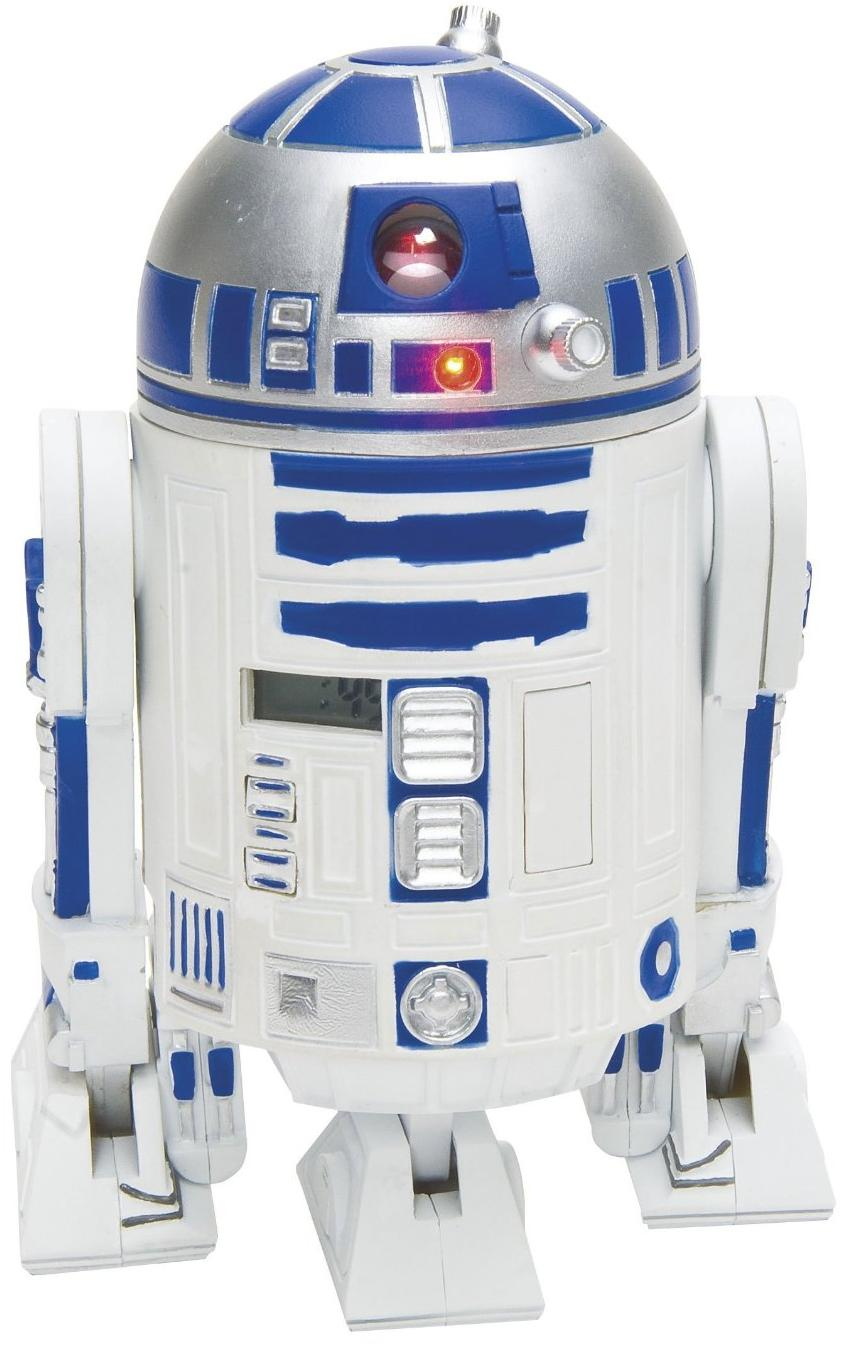
\includegraphics[height=4cm]{./img/near-dublicate-3-1.jpg}
        &
        %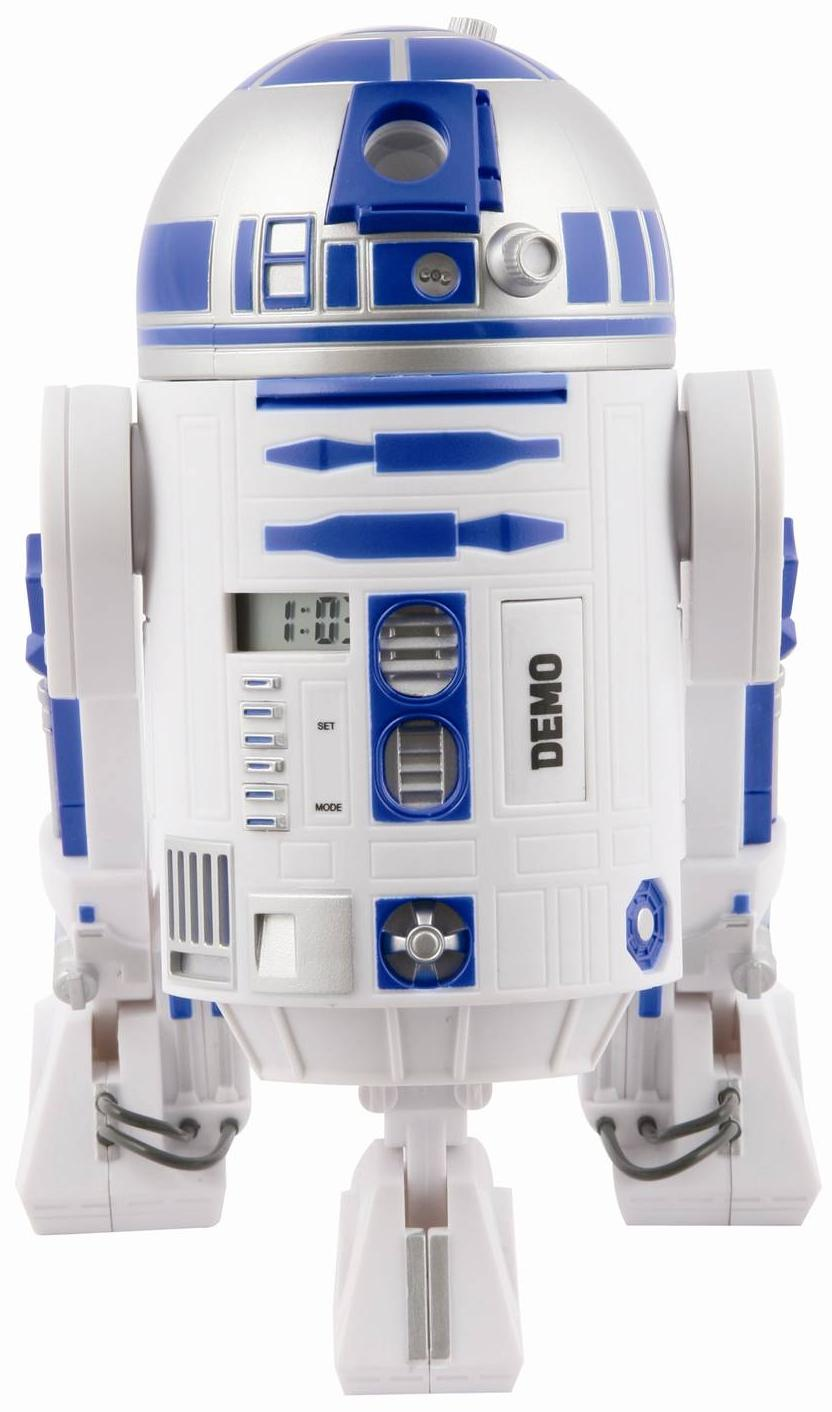
\includegraphics[height=4cm]{./img/near-dublicate-3-2.jpg}
        &
        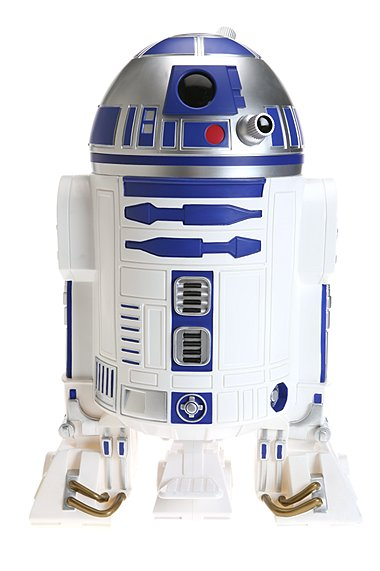
\includegraphics[height=4cm]{./img/near-dublicate-3-3.jpg}
        &
        %
\includegraphics[height=4cm]{./img/near-dublicate-3-4.jpg}
        &
        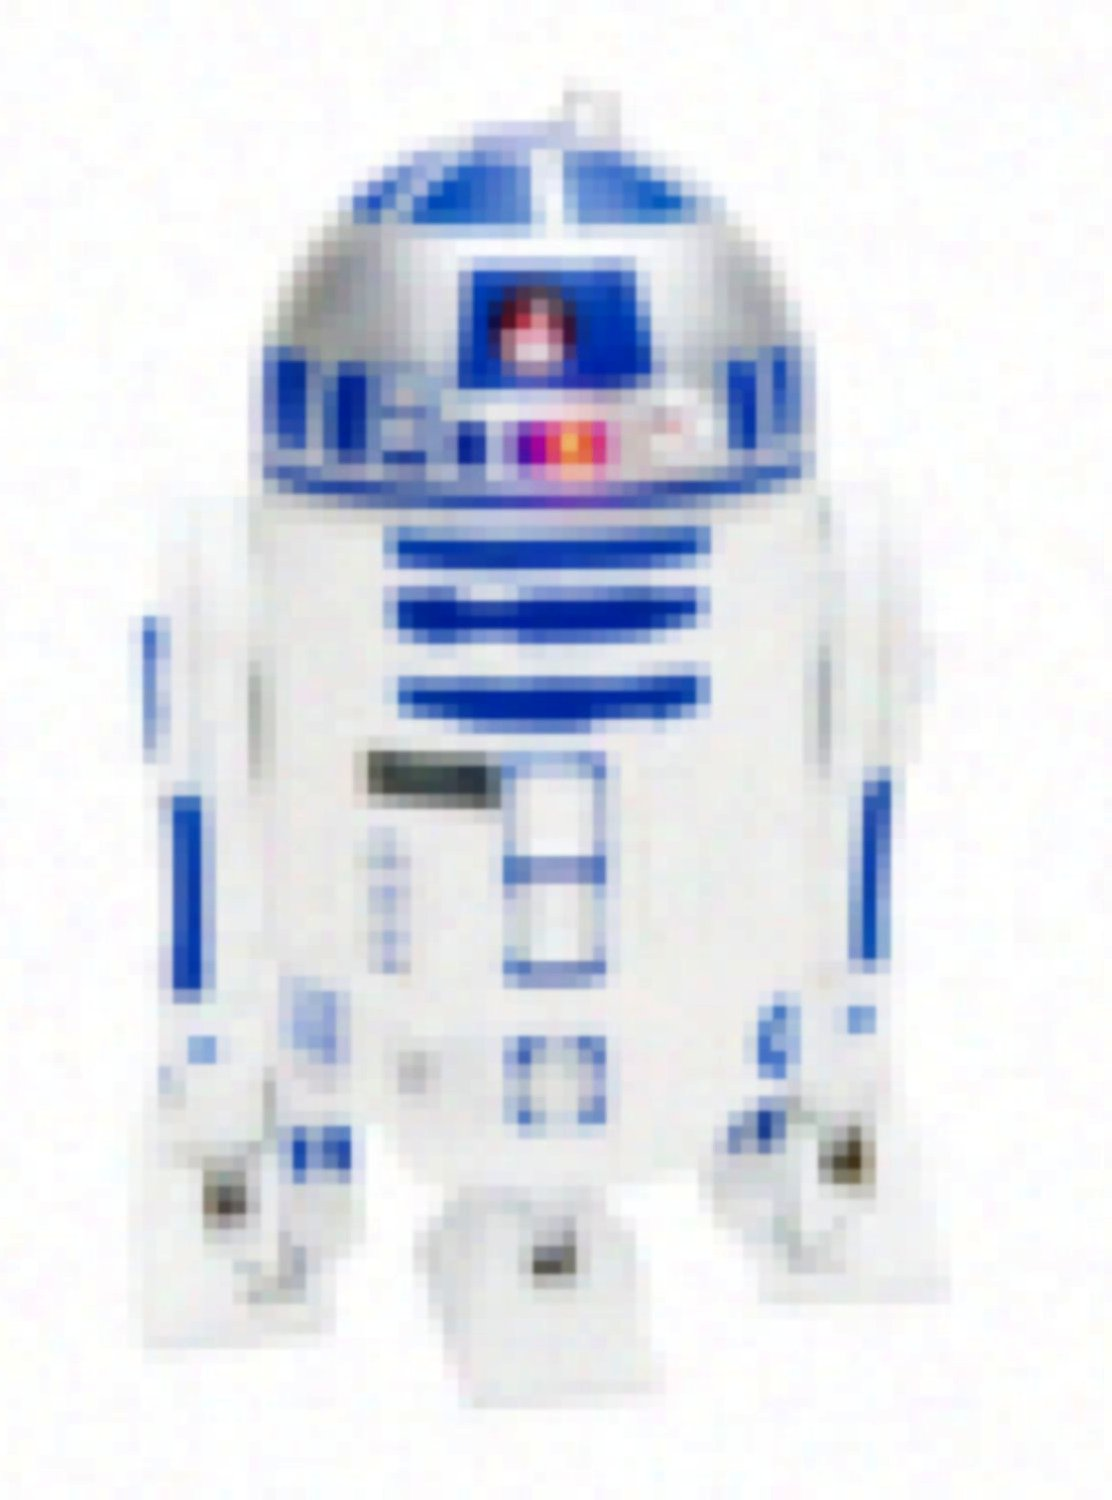
\includegraphics[height=4cm]{./img/near-dublicate-3-5.jpg}
        \\
        {\small оригинал}
        &
        %естественный дубликат
        &
        {\footnotesize естественный дубликат}
        &
        %искусственный дубликат
        &
        {\footnotesize искусственный дубликат}
        \\
    \end{tabular}
}

    

\subsection{Зачем}

\begin{frame}{Зачем искать <<нечеткие дубликаты>>}

\note{
    Поиск нечетких дубликатов может быть полезен
    для оптической навигации беспилотных аппаратов,
    для определения характера ландшфта местности,
    составления каталогов видео,
    группировки сниппетов поисковых систем,
    фильтрация видео рекламы
    и поиска пиратского видео.
}

    \begin{center}
        \begin{scriptsize}
            \tikzstyle{rootf} = [
                draw=yellow!50!black!70,thick,
                minimum height=1cm,
                minimum width=2cm,
                top color=yellow!20,
                bottom color=yellow!60!black!20,
                decorate,decoration={random steps,segment length=3pt,amplitude=1pt}
            ]
            \tikzstyle{pointf} = [
                rounded rectangle,
                thick,
                minimum size=1cm,
                draw=zdarkblue!50!black!50,
                top color=white,
                bottom color=zdarkblue!50!black!20
            ]
            \tikzstyle{milf} = [
                rectangle,
                thick,
                minimum size=1cm,
                draw=red!100!black!50,
                top color=white,
                bottom color=red!50!black!20
            ]
            \tikzstyle{submilf} = [
                rectangle, rounded corners,
                thick,
                minimum size=1cm,
                draw=red!70!black!50,
                top color=white,
                bottom color=red!30!black!20
            ]
            \tikzstyle{spacef} = [
                rectangle, rounded corners,
                thick,
                minimum size=1cm,
                draw=green!50!red!70!black!50,
                top color=white,
                bottom color=green!30!red!30!black!20
            ]
            \tikzstyle{orgf} = [
                rounded rectangle,
                thick,
                minimum size=1cm,
                draw=green!50!black!50,
                top color=white,
                bottom color=green!50!black!20
            ]
            \tikzstyle{catf} = [
                rounded rectangle,
                thick,
                minimum size=1cm,
                draw=green!70!red!10!black!50,
                top color=white,
                bottom color=green!70!red!10!black!20
            ]
            \tikzstyle{pirf} = [
                rounded rectangle,
                thick,
                minimum size=1cm,
                draw=green!50!black!50,
                top color=white,
                bottom color=green!50!black!20
            ]
            \tikzstyle{googlef} = [
                rounded rectangle,
                thick,
                minimum size=1cm,
                draw=green!70!blue!70!black!50,
                top color=white,
                bottom color=green!70!blue!70!black!20
            ]
            \tikzstyle{itemf} = [
                rectangle,thick,
                minimum width=2cm,
                minimum height=1cm,
                draw=teal!50!black!50,
                top color=white,
                bottom color=teal!50!black!20
            ]
            \begin{tikzpicture}[
                thick,node distance=2.5cm,
                text height=0.7ex,text depth=.25ex,
                auto
            ]
                \node[rootf] (all) {{\normalsize Цели}};
                \node[milf, below left of=all] (mil) {\footnotesize Военные};
                    \node[submilf, below left of=mil] (wr) {
                        \begin{tabular}{c}
                            {\tiny  оптическая навигация} \\
                            БПЛА \\
                        \end{tabular}
                    };
                    \node[spacef, below right of=mil] (space) {
                        \begin{tabular}{c}
                            определение \\
                            характера \\
                            поверхности
                        \end{tabular}
                    };
                \node[orgf, below right of=all] (org) {\footnotesize Мирные};
                    \node[catf,  below   of=org] (cat) {\scriptsize
                        \begin{tabular}{c}
                            cоставление \\
                            каталогов \\
                        \end{tabular}
                    };
                    \node[pirf, below right of=org] (pir) {
                        \begin{tabular}{c}
                            поиск \\
                            плагиата \\
                        \end{tabular}
                    };
                    \node[googlef, right of=org] (google) {
                        \begin{tabular}{c}
                            группировка  \\
                            сниппетов \\
                        \end{tabular}
                    };
                \path[->, red!100!black!50, very thick] (all) edge (mil);
                    \path[->, red!70!black!50, very thick] (mil) edge (wr);
                    \path[->, green!50!red!70!black!50, very thick] (mil) edge (space);
                \path[->, green!50!black!50, very thick] (all) edge (org);
                    \path[->, green!70!red!10!black!50, very thick] (org) edge (cat);
                    \path[->, green!50!black!50, very thick] (org) edge (pir);
                    \path[->, green!50!blue!70!black!50, very thick] (org) edge (google);
                    \path[->, green!50!red!70!black!50, very thick] (org) edge (space);
            \end{tikzpicture}
        \end{scriptsize}
    \end{center}
\end{frame}
    \subsection{Проблемы}

\frame{
    \frametitle{Связанные проблемы}

    \begin{center}
        \tikzstyle{nddf} = [
            rounded rectangle,
            thick,
            minimum size=1cm,
            draw=green!50!black!50,
            top color=white,
            bottom color=green!50!black!20
        ]
        \tikzstyle{classf} = [
            rounded rectangle,
            thick,
            minimum size=1cm,
            draw=blue!50!black!50,
            top color=white,
            bottom color=blue!50!black!20
        ]
        \tikzstyle{searchf} = [
            rounded rectangle,
            thick,
            minimum size=1cm,
            draw=red!50!black!50,
            top color=white,
            bottom color=red!50!black!20
        ]
        \begin{tikzpicture}[thick, node distance=3.0cm, text height=0.9ex, text depth=.25ex, auto]
            \node[nddf] (ndd) {Определение нечетких дубликатов};
            \node[classf,below left of=ndd] (class)  {Классификация видео};
            \node[searchf,below right of=class] (search) {Поиск по видео};
            \path[<->, green!50!black!50, very thick]   (ndd) edge (class);
            \path[<->, blue!50!black!50, very thick]    (class) edge (search);
            \path[<->, red!50!black!50, , very thick,decoration={zigzag,segment length=10,amplitude=1,
                            post=lineto,post length=2pt},font=\scriptsize,line join=round]  (ndd) edge[decorate] (search);
        \end{tikzpicture}
    \end{center}
}


  % Дубликаты
    \section{Решения}

    
\subsection{Cуществующие методы поиска}

\frame{
    \frametitle{Как пытаются искать}

        \begin{enumerate}
            \item  Сравние глобальных особенностей видео.
                {\tiny
                    \begin{itemize} \tiny
                        \item[${\color{zdarkblue} \vartriangleright}$]
                            функция яркости, функция визуального потока;
                        \item[${\color{zdarkgreen} +}$]
                            относительно быстро,
                            вычислительно просто;
                        \item[${\color{zdarkred} -}$]
                            легко обмануть.
                    \end{itemize}
                }
            \item  Сравние отдельных кадров и их сумм:
                {\tiny
                    \begin{itemize} \tiny
                        \item[${\color{zdarkblue} \vartriangleright}$]
                            глобальные особенности (гистограммы, спектры, GIST);
                        \item[${\color{zdarkblue} \vartriangleright}$]
                            локальные особенности (PCA-SIFT, детектор Харриса);
                        \item[${\color{zdarkgreen} +}$] точно;
                        \item[${\color{zdarkred} -}$] долго, затратно.
                    \end{itemize}
                }
            \item  Сравние звукового ряда
                (\href{http://youtube.com}
                    {\color{zdarkgreen}\it youtube.com}):
                {\tiny
                    \begin{itemize} \tiny
                        \item[${\color{zdarkgreen} +}$] быстро, просто;
                        \item[${\color{zdarkred} -}$] много ошибок,
                            не применимо если нет звука.
                    \end{itemize}
                }
            \item  Поиск и сравнение <<визуальных (видео) слов>>
                (\href{http://licenzero.ru}
                    {\color{zdarkgreen}\it licenzero.ru}):
                {\tiny
                    \begin{itemize} \tiny
                        \item[${\color{zdarkgreen} +}$] точно,
                            если достаточная база <<слов>>;
                        \item[${\color{zdarkred} -}$] долго,
                            нужно много размеченных данных.
                    \end{itemize}
                }
            \item  Комбинация методов.
        \end{enumerate}
        
}

    
\subsection{Предложение}

\begin{frame}{Алгоритм поиска нечетких дубликатов видео}
    \begin{itemize} \footnotesize
        \item $\nv$\ ---~новое видео;
        \item $\setsv = \{\sv[1], \sv[2], \dots, \sv[n]\}$\ ---~исходные видео:
            \begin{itemize}
                \item[${\color{zdarkblue}\leftarrow}$]
                    {\scriptsize  $\setsv$ может быть пустым};
                \item[${\color{zdarkblue}\leftarrow}$]
                    {\scriptsize для непустого $\setsv$
                        вычислены дескрипторы сцен элементов.}
            \end{itemize}
        \item[1.] Сравниваем дескриптор каждой
            сцены $\videoshot_{\color{red}\nv,i}$ из $\nv$\
            с дескриптором каждой сцены
            $\videoshot_{\color{red}\sv[k],j}$ из $\sv[k]$ в $L_2$.
        \item[2.] Если дескрипторы совпали $\nv$ c дескрипторами $\sv[k]$.
            на~некотором временном промежутке ,
            то считаем эту часть $\nv$\ ---~дубликатом $\sv[k]$,
            \begin{itemize}
                \item[] {\scriptsize несовпавшие
                    части $\nv$\ помещаем в $\setsv$}.
            \end{itemize}
        \item[3.] Если дескрипторы не совпали, то считаем $\nv$\ уникальным и
            добавляем в $\setsv$.
    \end{itemize}
\end{frame}


   % Решения
    \section{Сцены}

    
\subsection{Виды}

\begin{frame}[allowframebreaks]{Поиск на основе сцен}

    \orangebox{Кадр\ ---~{\it frame}, фотографический кадр}
    {\footnotesize
        \begin{itemize}
            \item[${\color{pacificorange} \Leftarrow}$]
                отдельная статическая картинка;
            \item[${\color{pacificorange} \Leftarrow}$]
                обозначим $\videoframe$.
        \end{itemize}
    }

    \vspace{12pt}
    \zgreenbox{Cъемка\ ---~{\it shot}, кинематографический кадр}
    {\footnotesize
        \begin{itemize}
            \item[${\color{zdarkgreen} \Leftarrow}$]
                множество фотографических кадров,
                единство процесса съемки;
            \item[${\color{zdarkgreen} \Leftarrow}$]
                обозначим $\videoshot$,
                $\videoframe \in \videoshot$;
            \item[${\color{zdarkgreen} \Leftarrow}$]
                часто называют <<сценой>>, 
                далее будем рассматривать, $\videoshot$, назвая сценой;
        \end{itemize}
    }
    \vspace{12pt}
    \zbluebox{Сцена\ ---~{\it scene}, монтажный кадр}
    {\footnotesize
        \begin{itemize}
            \item[${\color{zdarkblue} \Leftarrow}$]
                множество фотографических кадров,
                единство места и времени;
            \item[${\color{zdarkblue} \Leftarrow}$]
                обозначим $\videoscene$,
                $\videoframe \in \videoshot \subset \videoscene$.
        \end{itemize}
    }

    \zgreenbox{Сцена как <<съемка>>, кинематографический кадр}
    {
        ---~совокупность множества фотографических кадров $\videoframe$
        внутри временной области $\videoline$, кадры,
        которой $\videoframe_{\color{red} \videoshot, i}$
        значительно отличается от кадров соседних областей.
        \[
            \videoshot =
                \{
                    \videoframe_{\color{red} \videoshot, i}
                        | \videoframediff(\videoframe_{\color{red} \videoshot, i},
                            \videoframe_{\color{red} \videoshot, j})
                                < {\color{red} \varepsilon},
                            \videoframe_{\color{red} \videoshot, i},
                            \videoframe_{\color{red} \videoshot, j}
                            \in \videoline
                \}
        \]\[
            \videoframediff \text{\footnotesize \ ---~функция разности кадров}.
        \]
    }

    Аналогично можно ввести определение <<звуковой сцены>>,
    предварительно разделив звуковой сигнал на отсчеты.
\end{frame}

    
\subsection{Выделение}

\frame{
    \frametitle{Выделение cцен}

    %\begin{large}
        \begin{itemize}
            \item сравнение гистограмм яркости кадров;
            \vspace{10pt}
            \item сравнение спектров кадров;
            \vspace{10pt}
            \item сравнение векторов движения кадров.
        \end{itemize}
    %\end{large}

    \vspace{12pt}
    
    \begin{center}
        Первые кадры сцен рекламы МТС
        
\includegraphics[width=10cm]{./img/mts-scene.png}
    \end{center}
}

    
\subsection{Перемены сцен}

\frame[allowframebreaks]{
    \frametitle{Временные отметки перемены сцен}

    Временные отметки перемены сцен
    для видео закодированного различными кодеками.
    Замеры проводились при~низкой чувствительности.
    \begin{center}
        \large
        \begin{tabular}{|r|c|c|}
            \hline
            \multicolumn{3}{|c|}{\footnotesize Отметки в~секундах} \\
            \hline  $n$ &\textbf{vp6f}  & \textbf{h264}     \\
            \hline  $1$ & 0.094         & 0.04              \\
            \hline  $2$ &1.654          & 1.6               \\
            \hline  $3$ &6.574          & 6.52              \\
            \hline  $4$ &11.654         & 11.6              \\
            \hline  $5$ &14.254         & 14.2              \\
            \hline
        \end{tabular}
    \end{center}

    \framebreak

    Временные отметки перемены сцен
    для видео закодированного различными кодеками.
    Замеры проводились при~высокой чувствительности.
    \begin{center}
        \footnotesize
        \begin{tabular}{|r|c|c|c|}
            \hline
            \multicolumn{4}{|c|}{\footnotesize Отметки в~секундах} \\
            \hline $n$
                & \textbf{cinepak}
                &   \textbf{indeo5}
                &   \textbf{h264} \\
            \hline $1$  &0.133333   & 0.133333  & 0.133333  \\
            \hline $2$  &11.3333    & ---       & ---       \\
            \hline $3$  &74         & 74        & 74        \\
            \hline $4$  &78.9333    & ---       & ---       \\
            \hline $5$ &87.9333    & ---       & 87.9333   \\
            \hline $6$ &88.2667    & 88.2667   & 88.2667   \\
            \hline $7$ &88.3333    & ---       & ---       \\
            \hline $8$ &94.5333    & 94.5333   & 94.5333   \\
            \hline $9$ & ---       & 101.133   & 101.133   \\
            \hline $10$ &101.4      & ---       & 101.4     \\
            \hline $11$ &    ---    & ---       & 112       \\
            \hline
        \end{tabular}
    \end{center}
}

    
\subsection{Длины сцен}

\frame{
    \frametitle{Относительные длины}

    \begin{itemize}
        \item длина всех отрезков относительно всех,
        для рекламы МТС (для обоих вариантов) это будет представлять матрицу
        \[
            \left(
                \begin{matrix}
                    1.0000 & 0.3171 & 0.3071 & 0.6000 \\
                    3.1538 & 1.0000 & 0.9685 & 1.8923 \\
                    3.2564 & 1.0325 & 1.0000 & 1.9538 \\
                    1.6667 & 0.5285 & 0.5118 & 1.0000 \\
                \end{matrix}
            \right);
        \]
        \item длина отрезков относительно некоторых:
        \begin {itemize}
            \item[---] например $3$ предыдущих,
            \item[---] такой вариант применим для реального времени.
        \end{itemize}
    \end{itemize}
}

    
\subsection{Выравнивания}

\frame{
    \frametitle{Выравнивания длин}

    \vspace{20pt}
    \begin{tabular}{|r|l|l|l|l|l|l|l|}
        \hline  Время
            & 1 cек
            & 2 cек
            & 3 cек
            & 4 cек
            & 5 cек
            & 6 cек
            & 7 cек \\
        \hline
        \hline  Видео $v_1$
            & \multicolumn{2}{|l|}{ $\videoshot_{1, 1}$ }
            & \multicolumn{4}{|l|}{ $\videoshot_{1, 2}$ }
            &  $\videoshot_{1, 3}$\\
        \hline  Видео $v_2$
            & \multicolumn{6}{|l|}{ $\videoshot_{2, 1}$ }
            & $\videoshot_{2, 2}$ \\
        \hline
    \end{tabular}

    \vspace{12pt}
    
    Алгоритм Гейла-Черча для выравниваня длин предложений
    параллельных корпусов на разных языках
    \begin{itemize}
        \item требуется установить,
            что $v_1$ и $v_2$, <<переводы>> друг друга;
        \item когда лучше выравнивать, 
            {\it до} или {\it после} перехода к~относительным длинам:
            { \tiny
                \begin{itemize}
                    \item[до:] перевычислять относительные длины,
                    \item[после:] учитывать масштаб относительных длин;
                \end{itemize}
            }
        \item вычислительные затраты.
    \end{itemize}
    
%     Если длина текущей сцены одного видео меньше чем в 2 раза
%     длины текущей сцены другого видео, то текущую сцену первого видео
%     рассматривается вместе со следующей (алгоритм Гейла-Черча).

}
% 
% | . | . . . | |
% | . . . . . | |
% 
% 
% 1, 2, 0.5
% 1, 1.666

      % Cцены
    \section{Внутри сцены}

    
\subsection{Кадры}

\frame{
    \frametitle{При совпадени относительных длин сцен}

    \begin{itemize}
        \item нельзя делать вывод об одинаковости сцен;
        \item сравнить начальные и конечные кадры:
        \begin{itemize}
            \item[${\color{zdarkred}\bullet}$] сравнивать попиксельно или на основе <<знакового представления>> с разными масштабами:
                \begin{itemize}
                    \item[${\color{zdarkgreen} +}$] просто;
                    \item[${\color{zdarkred} -}$] не устойчиво к трансформациям.
                \end{itemize}
%             \item сравнивать на основе <<знакового представления>>:
%                 \begin{itemize}
%                     \item[${\color{zdarkgreen} +}$]
%                         вычислительно просто, устойчиво к трансформациям яркости;
%                     \item[${\color{zdarkred} -}$]
%                         не устойчиво к трансформациям направления и сдвигам,
%                         требует полного перебора направлений.
%                 \end{itemize}
            \item[${\color{zdarkred}\bullet}$] искать особенности в каждой паре кадров, SIFT:
                % \begin{itemize}
                %     \item вычисляем градиент в каждом пикселе
                %     \item строим гистограммы направлений градиентов по прямоугольным областям
                %     \item вклад каждого пикселя взвешиваем по гауссиане с центром в центре окрестности
                %     \item сравниваем как вектора в $L_2$
                % \end{itemize}
                \begin{itemize}
                    \item[${\color{zdarkgreen} +}$] надежно, устойчиво к искажениям;
                    \item[${\color{zdarkred} -}$] долго, для каждой пары сцен придется перевычислять особенности.
                \end{itemize}
            \item[${\color{zdarkgreen}\bullet}$] вычислить GIST для нужных кадров проверяемой cцены;
            \item[${\color{zdarkgreen}\bullet}$] воспользоваться <<мешком слов>> и МОВ.
        \end{itemize}
    \end{itemize}
При сравнении удобно иметь набор уже сопоставленных сцен.
}


    
\subsection{GIST}

\frame{
    \frametitle{GIST}
    Изначально используется для поиска похожих изображений.
    \vspace{12pt}
    \begin{enumerate}
        \item Считаем отклики детекторов краёв на~$5$~разных
            масштабах и~$6$~ориентациях края.
        \item Получаем $33$ <<канала>>\ ---~цвет и $30$ откликов фильтров края.
        \item Разобиваем изображение сеткой $4 \times 4$ на $16$ ячеек.
        \item В каждой ячейке усредняем значения всех каналов.
   \end{enumerate}
}
    \subsection{Мешок слов}

\frame{
    \frametitle{Мешок слов}
    Предполагаем, что есть некоторый набор изображений, на которых можно обучиться.
    
    \vspace{10pt}

    \zbluebox{Обучение}{
        \scriptsize
        \begin{itemize}
            \item[${\color{zdarkblue}\vartriangleright}$]
                собираем множество фрагментов (на основе SIFT);
            \item[${\color{zdarkblue}\vartriangleright}$]
                кластеризуем и строим словарь;
            \item[${\color{zdarkblue}\vartriangleright}$]
                квантуем каждый фрагмент по словарю;
            \item[${\color{zdarkblue}\vartriangleright}$]
                считаем <<мешки слов>> для каждого изображения;
            \item[${\color{zdarkblue}\vartriangleright}$]
                обучаем МОВ на мешках слов.
        \end{itemize}
    }
    
    \vspace{10pt}

    \zgreenbox{Сопоставление}{
        \scriptsize
        \begin{itemize}
            \item[${\color{zdarkgreen}\vartriangleright}$]
                выбираем фрагменты из изображения (на основе SIFT);
            \item[${\color{zdarkgreen}\vartriangleright}$]
                квантуем каждый фрагмент по словарю;
            \item[${\color{zdarkgreen}\vartriangleright}$]
                строим <<мешок слов>> для изображения;
            \item[${\color{zdarkgreen}\vartriangleright}$]
                применяем классификатор МОВ.
        \end{itemize}
    }
}





    \subsection{Дескриптор сцены}

\frame{
    \frametitle{Дескриптор сцены}



    \def\drawdescrpicture{
        \begin{center}
        \begin{scriptsize}
        \tikzstyle{rootf} = [
            draw=yellow!50!black!70,thick,
            minimum height=2cm,
            minimum width=2cm,
            top color=yellow!20,
            bottom color=yellow!60!black!20,
            decorate,decoration={random steps,segment length=3pt,amplitude=1pt}
        ]

        \tikzstyle{pointf} = [
            rectangle, rounded corners,
            thick,
            minimum size=1cm,
            draw=zdarkblue!50!black!50,
            top color=white,
            bottom color=zdarkblue!50!black!20
        ]

        \tikzstyle{shotf} = [
            rectangle, rounded corners,
            thick,
            minimum size=1.5cm,
            draw=red!100!black!50,
            top color=white,
            bottom color=red!50!black!20
        ]

        \tikzstyle{subshotf} = [
            rectangle, rounded corners,
            thick,
            minimum size=1cm,
            draw=red!70!black!50,
            top color=white,
            bottom color=red!30!black!20
        ]


        \tikzstyle{spacef} = [
            rectangle, rounded corners,
            thick,
            minimum size=1cm,
            draw=green!50!red!70!black!50,
            top color=white,
            bottom color=green!30!red!30!black!20
        ]

        \tikzstyle{framef} = [
            rectangle, rounded corners,
            thick,
            minimum size=1.5cm,
            draw=green!50!black!50,
            top color=white,
            bottom color=green!50!black!20
        ]

        \tikzstyle{bowf} = [
            rectangle, rounded corners,
            thick,
            minimum size=1cm,
            draw=green!70!red!10!black!50,
            top color=white,
            bottom color=green!70!red!10!black!20
        ]

        \tikzstyle{gistf} = [
            rectangle, rounded corners,
            thick,
            minimum size=1cm,
            draw=green!50!black!50,
            top color=white,
            bottom color=green!50!black!20
        ]


        \tikzstyle{googlef} = [
            rectangle, rounded corners,
            thick,
            minimum size=1cm,
            draw=green!70!blue!70!black!50,
            top color=white,
            bottom color=green!70!blue!70!black!20
        ]


        \tikzstyle{itemf} = [
            rectangle,thick,
            minimum width=2cm,
            minimum height=2cm,
            draw=teal!50!black!50,
            top color=white,
            bottom color=teal!50!black!20
        ]
        \begin{tikzpicture}[thick, node distance=2.5cm, text height=0.7ex, text depth=.25ex, auto]

            \node[pointf] (all) {{\normalsize Дескриптор}};
            \node[shotf, below left of=all] (shot) {\footnotesize
                \begin{tabular}{c}
                    отношения длины \\
                    сцены к~длинам \\
                    других сцен \\
                \end{tabular}
            };
                \node[subshotf, above left of=shot] (subshot) {\scriptsize
                    \begin{tabular}{c}
                        удобно хранить, \\
                        с~объединениями \\
                        соседних сцен \\
                    \end{tabular}
                };
                \node[spacef, below of=subshot] (space) {\tiny
                    \begin{tabular}{c} %% для длин \\
                        по $3$ предыдущим \\
                        \ ---~$6$~вариантов.
                    \end{tabular}
                };

            \node[framef, below right of=all] (frame) {\footnotesize
                \begin{tabular}{c}
                    Xарактеристики \\
                    {\scriptsize начального и конечного} \\
                    кадров \\
                \end{tabular}
            };

                \node[bowf,  below   of=frame] (bow) {\scriptsize
                    \begin{tabular}{c}
                        {\tt\color{red} или} \\
                        <<мешки слов>> \\
                    \end{tabular}
                };

                    \node[bowf,  below of=bow] (bowplus) {\tiny
                        \begin{tabular}{c}
                            лучше соответвует \\
                            предметной области\\
                        \end{tabular}
                    };

                \node[gistf, below right of=frame] (gist) {\scriptsize
                    \begin{tabular}{c}
                        {\tt\color{red} или} \\
                        GIST \\
                    \end{tabular}
                };
   

            \path[->, red!100!black!50, very thick] (all) edge (shot);
                \path[->, red!70!black!50, very thick] (shot) edge (subshot);
                \path[->, green!50!red!70!black!50, very thick] (subshot) edge (space);


            \path[->, green!50!black!50, very thick] (all) edge (frame);
                \path[->, green!70!red!10!black!50, very thick] (frame) edge (bow);
                \path[->, green!50!black!50, very thick] (frame) edge (gist);


        \end{tikzpicture}
        \end{scriptsize}
        \end{center}
    }

    %\drawdescrpicture

    \begin{enumerate}
        \item Вектор отношений длины сцены к длинам других сцен;
            \begin{itemize}
                \item удобно сразу хранить, с объединениями соседних сцен;
                \item для относительных длин
                    по трем предыдущим\ ---~$6$~вариантов.
            \end{itemize}
        \vspace{6pt}
        \item Xарактеристики начального и конечного кадров:
        \begin{itemize}
            \item или <<мешки слов>> начального и конечного кадров:
            \begin{itemize}
                \item[${\color{zdarkgreen}+}$] лучше соответвует предметной области,
                \item[${\color{zdarkred}-}$] потенциально бесконечный размер вектора гистограммы;
            \end{itemize}
            \item или GIST начального и конечного кадров;
            \begin{itemize}
                \item[${\color{zdarkgreen}+}$] не требует какого либо обучения,
                \item[${\color{zdarkred}-}$] менее точен.
            \end{itemize}
        \end{itemize}
    \end{enumerate}
%     \vspace{12pt}
%     \begin{itemize}
%         \item[${\color{red}\Rightarrow}$] объемный вектор, сравнивать не удобно.
%     \end{itemize}
}

% 
% | 1| 2|x3|
% | 1   |x3|
% | 2   |x3|
% | 1|   x3|
% | 2|   x3|
% |      x3|


% Rather than using random projections to define the bits in a code, several authors have
% pursued machine learning approaches. In [5] the authors used an autoencoder with several
% hidden layers. The architecture can be thought of as a restricted Boltzmann machine (RBM)
% in which there are only connections between layers and not within layers. In order to learn 32
% bits, the middle layer of the autoencoder has 32 hidden units, and noise was injected during
% training to encourage these bits to be as binary as possible. This method indeed gives codes
% that are much more compact than the E2LSH codes. In [9] they used multiple stacked RBMs
% to learn a non-linear mapping between input vector and code bits. Backpropagation using
% an Neighborhood Components Analysis (NCA) objective function was used to refine the
% weights in the network to preserve the neighborhood structure of the input space. Figure 1
% shows that the RBM gives much better performance compared to random bits. A simpler
% machine learning algorithm (Boosting SSC) was pursued in [10] who used adaBoost to
% classify a pair of input items as sishotar or nonsishotar. Each weak learner was a decision
% stump, and the output of all the weak learners on a given output is a binary code. Figure 1
% shows that this boosting procedure also works much better than E2LSH codes, although
% slightly worse than the RBMs1
% .


    % Внутри сцены
    \section{Алгоритм}

    \subsection{Алгоритм}



\frame{
    \frametitle{Алгоритм поиска нечетких дубликатов видео}
    {     
    \begin{itemize} \footnotesize
        \item $\nv$\ ---~новое видео;
        \item $\setsv = \{\sv[1], \sv[2], \dots, \sv[n]\}$\ ---~исходные видео:
            \begin{itemize}
                \item[${\color{zdarkblue}\leftarrow}$]
                    {\scriptsize  $\setsv$ может быть пустым};
                \item[${\color{zdarkblue}\leftarrow}$]
                    {\scriptsize для непустого $\setsv$
                        вычислены дескрипторы сцен элементов.}
            \end{itemize} 
        \item[1.] Сравниваем дескриптор каждой
            сцены $\videoshot_{\color{red}\nv,i}$ из $\nv$\
            с дескриптором каждой сцены
            $\videoshot_{\color{red}\sv[k],j}$ из $\sv[k]$ в $L_2$.
        \item[2.] Если дескрипторы совпали $\nv$ c дескрипторами $\sv[k]$.
            на~некотором временном промежутке ,
            то считаем эту часть $\nv$\ ---~дубликатом $\sv[k]$,
            \begin{itemize}
                \item[] {\scriptsize несовпавшие
                    части $\nv$\ помещаем в $\setsv$}.
            \end{itemize}
        \item[3.] Если дескрипторы не совпали, то считаем $\nv$\ уникальным и
            добавляем в $\setsv$.
    \end{itemize}
    \vspace{4pt}
    \begin{itemize}
        \item[${\color{zdarkred}(-)}$] Cравнивать дескрипторы явно\ ---~не эффективно,
        \begin{itemize}
            \item[] {\scriptsize можно применить семантическое хеширование}.
        \end{itemize}
    \end{itemize}
    }
}


\subsection{Семантическое хеширование}

\frame{
    \frametitle{Семантическое хеширование}
    \begin{itemize}
        \item Введем бинарные подписи.
            \vspace{10pt}
        \item Подписи для близких в $L_2$ сцен должны быть близки.
            \vspace{10pt}
        \item  Локально чувстивтельное хеширование:
            \begin{enumerate}
                \item  Cлучайная проекция данных на прямую.
                \item  Случайно выберем порог,
                    пометив проекции $0$ или $1$.
                \item  С увеличением числа бит подпись
                    приближает $L_2$-метрику в исходных дескрипторах.
            \end{enumerate}
            \vspace{10pt}
        \item  Обучаемое хеширование.
    \end{itemize}
}

\subsection{Обучаемое хеширование}

\frame{
    \frametitle{Обучаемое хеширование}


    \bluebox{Cтимулирование (boosting)}
    {\footnotesize
        \begin{itemize}
            \item[$\Leftarrow$] BoostSSC;
            \item[$\Leftarrow$] Расстояние между дескрипторами вычисляется,
                как расстояние Хемминга.
        \end{itemize}
    }
    \vspace{12pt}
    \orangebox{Ограниченная машина Больцмана}
    {\footnotesize
        \begin{itemize}
            \item[${\color{pacificorange}\Leftarrow}$] связь только между слоями;
            \item[${\color{pacificorange}\Leftarrow}$] внутри слоев связи нет;
            \item[${\color{pacificorange}\Leftarrow}$]
                мощность слоев понижается от размера входного
                вектора до размера требуемого кода.
        \end{itemize}

    }
%     
%     \begin{enumerate}
%         \item  Cтимулирование (boosting).
%         \begin{itemize}
%             \item  BoostSSC;
%             \item  Расстояние между дескрипторами вычисляется, 
%                 как расстояние Хемминга
%         \end{itemize}
%         \item  C использованием ограниченной машины Больцмана:
%         \begin{itemize}
%             \item  связь только между слоями;
%             \item  внутри слоев связи нет;
%             \item  мощность слоев понижается от размера входного
%                 вектора до размера требуемого кода;
%         \end{itemize}
%     \end{enumerate}
}

\section{Результаты}

\subsection{Результаты и перспективы}

\frame{
    \frametitle{Результаты и перспективы}
    {\color{zdarkgreen} Результаты}:
        { \footnotesize
            \begin{itemize}
                \item предложен подход:
                \begin{itemize}
                    \item[${\color{zdarkblue}\vartriangleright}$] {\scriptsize относительные длины},
                    \item[${\color{zdarkblue}\vartriangleright}$] {\scriptsize выравнивания},
                    \item[${\color{zdarkblue}\vartriangleright}$] {\scriptsize дескрипторы сцен};
                \end{itemize}
                \item проведены эксперименты.
            \end{itemize}
        }
        \vspace{12pt}
    {\color{zdarkgreen} Дальнейшее развитие}
        { \footnotesize
            \begin{itemize}
                \item изменить алгоритм поска перемены сцены,
                    \begin{itemize}
                        \item[$\vartriangleright$] {\scriptsize сейчас используется {\tt ffmpeg}};
                    \end{itemize}
                \item хеширование на основе машины Больцмана;
                \item эксперименты на реальном множестве исxодных данных.
            \end{itemize}
        }
}

% 
%  \scriptsize
%     \begin{codebox}
%         \Procname{Базовый-алгоритм($\TE$, $\TR$)}
%         \li     $\forall \ \WE \in \SE \in \TE $ \Do
%         \li         $\forall \WR \in \SR \in \TR $ \Do
%         \li             $ t(\WE|\WR) \gets u, u \in \mathbb{R}$;
%                     \End
%                 \End
%         \li     \Com{ Инициализируем таблицу $t(\WE|\WR)$ одинаковыми значениями.}
%         \li     \Пока {не сойдется} \Do
%         \li         $\forall \ \WE \in \SE \in \TE $ \Do \Com{ Инициализируем остальные таблицы.}
%         \li             $\forall \WR \in \SR \in \TR $ \Do
%         \li                 $ counts(\WE|\WR) \gets  0$;  $\quad total(\WR) \gets  0$;
%                         \End
%                     \End
%         \li         $\forall \ \SE, \SR \in \TE, \TR$ \Do \Com{ Вычисляем нормализациию. }
%         \li             $\forall \ \WE \in \SE$ \Do
%         \li                 $stotal(\WE) \gets  0$;
%         \li                 $\forall \ \WR \in \SR$ \Do
%         \li                     $stotal(\WE) \gets stotal(\WE) + t(\WE|\WR)$;
%                             \End
%                         \End
%         \li             $\forall \ \WE \in \SE$ \Do \Com{ Собираем подсчеты. }
%         \li                 $\forall \ \WR \in \SR$ \Do
%         \li                     $counts(\WE|\WR) \gets counts(\WE|\WR) + \dfrac{t(\WE|\WR)}{stotal(\WE)}$;
%         \li                     $total(\WR) \gets total(\WR) + \dfrac{t(\WE|\WR)}{stotal(\WE)}$;
%                             \End
%                         \End
%                     \End
%         \li         $\forall \ \WE \in  \TE $ \Do \Com{ Оцениваем вероятность.}
%         \li             $\forall \WR \in \TR $ \Do
%         \li                 $ t(\WE|\WR) \gets \dfrac{counts(\WE|\WR)}{total(\WR)}$;
%                         \End
%                     \End
%                 \End
%     \end{codebox}
    %\subsection{Оптимизация}

\frame{
    \frametitle{Выравнивания длин}

    \vspace{20pt}
    \begin{tabular}{|r|l|l|l|l|l|l|l|}
        \hline  Время
            & 1 cек
            & 2 cек
            & 3 cек
            & 4 cек
            & 5 cек
            & 6 cек
            & 7 cек \\
        \hline
        \hline  Видео $v_1$
            & \multicolumn{2}{|l|}{ $\videoshot_{1, 1}$ }
            & \multicolumn{4}{|l|}{ $\videoshot_{1, 2}$ }
            &  $\videoshot_{1, 3}$\\
        \hline  Видео $v_2$
            & \multicolumn{6}{|l|}{ $\videoshot_{2, 1}$ }
            & $\videoshot_{2, 2}$ \\
        \hline
    \end{tabular}

    \vspace{12pt}

    Алгоритм Гейла-Черча для выравниваня длин предложений
    параллельных корпусов на разных языках
    \begin{itemize}
        \item требуется установить,
            что $v_1$ и $v_2$, <<переводы>> друг друга;
        \item когда лучше выравнивать,
            {\it до} или {\it после} перехода к~относительным длинам:
            { \tiny
                \begin{itemize}
                    \item[до:] перевычислять относительные длины,
                    \item[после:] учитывать масштаб относительных длин;
                \end{itemize}
            }
        \item вычислительные затраты.
    \end{itemize}

%     Если длина текущей сцены одного видео меньше чем в 2 раза
%     длины текущей сцены другого видео, то текущую сцену первого видео
%     рассматривается вместе со следующей (алгоритм Гейла-Черча).

}

   % Алгоритм

\end{document}


